\documentclass[12pt]{exam}
\usepackage[utf8]{inputenc}
\usepackage[T1]{fontenc}
\usepackage{wrapfig}
\usepackage{amsmath}
\usepackage{amssymb}
\usepackage{hyperref}
\usepackage{graphicx}
\usepackage[norsk]{babel}
\usepackage{tikz}
\usepackage{tkz-euclide}
\usepackage{float}
\usepackage{wrapfig}
\usepackage{pgfplots}
\pgfplotsset{compat=1.11}


\begin{document}
\qformat{\underline{Spørsmål \thequestion} \hfill}


\begin{questions}
  
\question Regn ut kryssproduktet $\vec{p} \times \vec{q}$\\
\begin{parts}
\begin{minipage}{0.5\textwidth}
\part 
\begin{align*}
\vec{p} &= [1,1,1]\\
\vec{q} &= [1,2,3]
\end{align*}
\part 
\begin{align*}
\vec{p} &= [1,2,1]\\
\vec{q} &= [1,5,3]
\end{align*}
\end{minipage}%
\begin{minipage}{0.45\textwidth}
\part 
\begin{align*}
\vec{p} &= [1,0,2] \\
\vec{q} &= [-2,1,3]
\end{align*}
\part 
\begin{align*}
\vec{p} &= [2,1,0] \\
\vec{q} &= [3,1,1]
\end{align*}
\end{minipage}%
\end{parts}

\question Du har to vektorer $\vec{p}$ og $\vec{q}$ med en vinkel immellom dem på $\frac{\pi}{6}$. 
Vi vet at $|\vec{p}| = 2$ og at $|\vec{q}| = 3$. Hva er da $|\vec{p} \times \vec{q}|$?


\question Du har to vektorer $\vec{p}$ og $\vec{q}$ med en vinkel immellom dem på $\frac{\pi}{4}$. 
Vi vet at $|\vec{p}| = 3$ og at $|\vec{q}| = 7$. Hva er da $|\vec{p} \times \vec{q}|$?

\begin{minipage}{0.5\textwidth}
\question Bruk kryssproduktet til å finne arealet av trekanten.
\end{minipage}%
\begin{minipage}{0.5\textwidth}
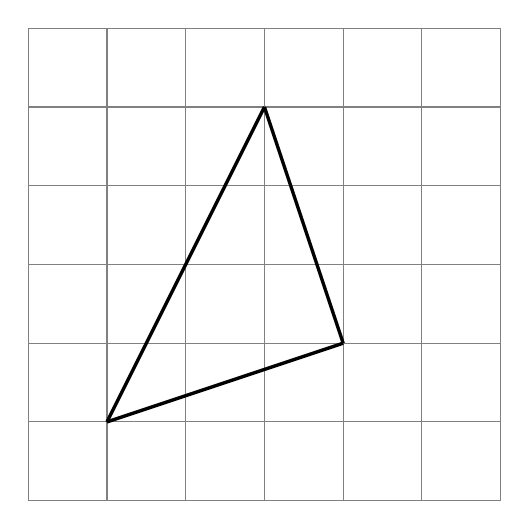
\begin{tikzpicture}[scale = 1.0,every node/.style={scale=1.0}]
\tkzInit[xmin=-1,xmax=5,ymin=-1,ymax=5]
\tkzGrid[color=gray]
\tkzAxeXY[very thick]
\draw[black,very thick] (3,1) -- (2,4);
\draw[black,very thick] (3,1) -- (0,0);
\draw[black,very thick] (2,4) -- (0,0);
--cycle;
\end{tikzpicture}  
\end{minipage}%


\question
\begin{parts}
\part Finn $t$ slik at $[2,1,t] \times [4,3,2] \perp [3,2,1]$
\part Finn $t$ slik at $[2,1,t] \times [3,4,5 ]\; ||  \;[1,-1,1]$
\part Finn $t$ slik at $|\vec{n}| = \sqrt{3}$ når
\[
\vec{n} = [2,1,t] \times [2,3,1]
\]
\end{parts}

\question Forklar hvorfor for to vektorer $\vec{p},\vec{q}$ så har vi alltid at:
\[
(\vec{p} \times \vec{q}) \cdot \vec{p} = 0.
\]


\end{questions}







\end{document}